% Install the following packages: beamer, xcolor and pgm

\documentclass[]{beamer}
\mode<presentation>{
 \usetheme{Rochester}			% schlichtes, blaues theme
 \setbeamercovered{transparent}		% Schattieren des verborgenen Textes
}
\usepackage[T1]{fontenc}
\usepackage[utf8]{inputenc}		% Support german umlauts
\usepackage[ngerman]{babel}		% Print german date
%\usepackage{pgfpages}			% Ausdruck auf mehrere Seiten
%\pgfpagesuselayout{4 on 1}[a4paper,landscape,border shrink=5mm]
\usepackage{graphicx}			% Graphiken benutzen

\pgfdeclareimage[height=1.5cm]{logo}{../src/img/splash}	% Logo rechts unten anzeigen
\logo{\pgfuseimage{logo}}

\title{Miniprojekt UserInterfaces -- Schlusspräsentation}
\author{Thomas Kallenberg, Martin Schwab}
\institute{HSR Hochschule Rapperswil}
\date{ \today }

\begin{document}

\begin{frame}
  \titlepage
\end{frame}

\begin{frame}{Übersicht}
\begin{itemize}
\item Was wurde umgesetzt
\item Demo
\item Technische Hintergründe
\item Fazit
\end{itemize}
\end{frame}

\begin{frame}{Was wurde umgesetzt}
 \begin{itemize}
   \item Liste mit eigener Suche
   \item Statuszeile mit Statistik
   \item Sortierung Suchresultate
   \item Aufgabenorientierte CellRenderer
   \item Splash...
   \item Projektautomatisierung
 \end{itemize}
\end{frame}

\begin{frame}{Demonstration}
\begin{columns}[t]
  \begin{column}{5cm}
   \begin{itemize}
    \item (Demo-)User aktivieren
    \item Buchausleihe gesperrt :-(
    \item Rückgabe überfälliges
    \item Buchausleihe möglich
    \item Benutzerdetails editieren
   \end{itemize}
  \end{column}
  \begin{column}{5cm}
   \begin{figure}
     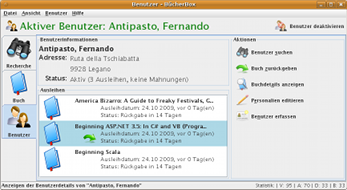
\includegraphics[scale=0.4]{screen}
     \caption{Benutzerdetails}
   \end{figure}
  \end{column}
\end{columns}
\end{frame}

\begin{frame}{Technische Hintergünde}{Suchfunktion}
\begin{itemize}
\item<1-> Jeder Tastenanschlag wird weitergeleitet
  \begin{itemize}
  \item<2-> ein neues Zeichen wird angefügt
      \begin{itemize}
	\item<3-> letztes Suchresultat speichern, auf dessen Basis Anzeige weiter einschränken
      \end{itemize}
    \item<4-> das letzte Zeichen wird gelöscht
      \begin{itemize}
	\item<5-> vorletztes gespeichertes Suchresultat wird an die Stelle des aktuellen Resultats gesetzt
      \end{itemize}
  \end{itemize}
\item<6-> Ggf. Zwischenresultate neu aufbauen: Langsam aber selten
\item<7-> Bibliothek geändert $\rightarrow$ neu aufbauen
\item<8-> Suche fertig  $\rightarrow$  Liste per Observer informieren
\invisible<1-8>{ \item . }
\end{itemize}
\end{frame}

\begin{frame}{Erkenntnisse}
\begin{itemize}
 \item Grafische Elemente wie verbinden? \\ $\rightarrow$ Architekturwissen fehlte
 \item kleine, wichtige Details = viel Zeit % FocusTraversalPolicy über mehrere Panels...
 \item GUI-Refactoring schwierig
 \item Kleine Werbepause: git und github.com :-)
\end{itemize}
\end{frame}

\end{document}
